\documentclass[title-dark, color-primary=tubaf-primary-dark]{tubaf-beamer}

\usepackage{adjustbox}
\usepackage[sans]{tubaf-fonts}
\usepackage[english]{babel}
\usepackage{imf-logo}
\usepackage{tikz}
\usepackage{tabularray}
\usepackage[style=authoryear, maxnames=1]{biblatex}
\addbibresource{refs.bib}
\usepackage{unicode-math}
\usepackage{symbols}
\usepackage{qrcode}
\usepackage[mode=match]{siunitx}
\usepackage{multicol}
\usepackage{animate}

\AtBeginPart{\frame{\partpage}}
\AtBeginSection{\frame{\sectionpage}}
\AtBeginSubsection{\frame{\subsectionpage}}
\setbeamercolor*{button}{parent=palette primary}
\setbeamercolor*{button border}{parent=palette primary}
\addtobeamertemplate{headline}{}{\hfill\hyperlink{contents}{\beamerbutton{CNT}} \hyperlink{appendix-contents}{\beamerbutton{APP}}}
\newenvironment{alertblockenv}{\only{\setbeamercolor*{block title}{fg=white,bg=palette secondary.fg,use=palette secondary}\setbeamercolor*{block body}{bg=block title.bg!15!white,use=block title}}}{}

\contact{%
    \begin{columns}[b]
        \begin{column}{0.72\textwidth}
            Max Weiner\\
            Institute of Metal Forming\\
            TU Bergakademie Freiberg\\
            Bernhard-von-Cotta-Str. 4\\
            DE-09599 Freiberg\\
            Phone: 049 3731 39 2952\\
            Mail: max.weiner@imf.tu-freiberg.de
        \end{column}
        \begin{column}{0.28\textwidth}
            \qrcode[height=\linewidth]{MECARD:N:Weiner,Max;TEL:+49\ 3731\ 392952;EMAIL:max.weiner@imf.tu-freiberg.de;;}
            \vspace{0pt}
        \end{column}
    \end{columns}
}

\begin{document}
\title{Microscopic Simulation of Solid State Sintering Regarding Irregularly Shaped Powder Particles}
\subtitle{Defense of Doctoral Thesis}
\author[Max Weiner]{Max Weiner}
\logo{\imflogo}
\logowhite{\imflogomono[fill=white]}
\titlegraphic{\includegraphics{img/title_bw}}
\date{2025-10-13}
\institute{Institute of Metal Forming, TU Bergakademie Freiberg}

\begin{frame}[plain,noframenumbering]
    \maketitle
\end{frame}

\begin{frame}[label=contents]{Contents}
    \tableofcontents

    % \begin{tikzpicture}[overlay, remember picture]
    %     \useasboundingbox (current page.south west) rectangle(current page.north east);
    %     \begin{scope}[on background layer]
    %         \tubaftrapezoidright*[path picture={
    %                 \node at (path picture bounding box.center) {
    %                     \includegraphics[height=1.1\paperheight]{img/title}
    %             };}
    %         ]{8cm};
    %     \end{scope}
    % \end{tikzpicture}
\end{frame}

\section{Introduction}

\begin{frame}{Definition of Sintering}
    \begin{block}{Sintering}
        \begin{itemize}
            \item  Is a heat treatment process to alter microstructure of powder compacts for achieving certain properties (mainly mechanical strength).
            \item Is a thermodynamically voluntary process driven by reduction of energy stored in defects (especially surfaces and grain boundaries).
        \end{itemize}
    \end{block}
    \medskip
    \structure{The system is in non-equilibrium thermodynamic state and evolves towards equilibrium (seldom ever reaching it).}
\end{frame}

% \begin{frame}{The Laws of Thermodynamics}
    \begin{quote}
        The laws of thermodynamics:
        \begin{enumerate}
            \item You can not win.
            \item You can not break even.
            \item You can not get out of the game.
        \end{enumerate}

        \hfill --- Unknown
    \end{quote}

    \only<2>{%
        \medskip
        \begin{block}{The Actual Axioms}
            \begin{enumerate}
                \item Energy can neither be created nor destroyed.
                \item The overall entropy stays constant or increases (irreversible processes).
                \item The entropy of a perfect crystal at \qty{0}{\kelvin} is \qty{0}{\joule\per\kelvin}.
            \end{enumerate}
        \end{block}
    }
\end{frame}

\begin{frame}{Equilibrium vs. Non-Equilibrium Thermodynamics}
    \begin{block}{Equilibrium}
        \begin{itemize}
            \item The equilibrium state of a system is characterized by a minimum of the corresponding thermodynamic potential (or a maximum of overall entropy).
            \item A system outside equilibrium will voluntarily change its state approaching the equilibrium.
        \end{itemize}
    \end{block}

    \begin{description}
        \item[\alert{Problem}] Entropy and temperature are only well-defined in equilibrium.
        \item[Attempts]\hfill
            \begin{itemize}
                \item Assuming a local equilibrium state (or accompanying equilibrium state).
                \item Just assuming the validity of those definitions outside equilibrium.
            \end{itemize}
    \end{description}
\end{frame}

\begin{frame}{Internal Variables of State}
    \begin{block}{Variables of State}
        \begin{itemize}
            \item Natural variables of the thermodynamic potentials: $\Temperature$ or $\Entropy$, $\Pressure$ or $\Volume$, $\Substance$ or $\ChemicalPotential$.
            \item Define the macroscopic state of the system.
            \item Measurable and controllable.
        \end{itemize}
    \end{block}

    \begin{block}{Internal Variables of State}
        \begin{itemize}
            \item Arbitrary variables characterizing microscopic state at arbitrary level of detail.
            \item Account for \emph{our lack of knowledge} about microstructural state of the system.
            \item May be measurable, but usually out of direct control.
        \end{itemize}
    \end{block}
\end{frame}

\begin{frame}{Encouragement}
    \begin{quote}
        Perhaps, after all, the wise man's attitude towards thermodynamics should be to have nothing to do with it. To deal with thermodynamics is to look for trouble.

        \hfill --- \textcite{Maugin1999}
    \end{quote}
\end{frame}


\section{State of the Art}

\begin{frame}{Sintering Models}
    \begin{columns}[t]
        \begin{column}{0.5\linewidth}
            \structure{Microscopic Models}
            \begin{itemize}
                \item Regard distinct particles.
                \item Model diffusional fluxes and evolution of particle shape.
            \end{itemize}
            \vspace{1ex}
            \centering
            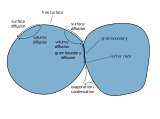
\includegraphics[width=60mm]{img/basic_theory//diffusion_mechanisms}
        \end{column}
        \begin{column}{0.5\linewidth}
            \structure{Macroscopic Models}
            \begin{itemize}
                \item Regard components consisting of "continuous" material.
                \item Model densification, stresses and strains.
            \end{itemize}
            \vspace{1ex}
            \centering
            \includegraphics[width=30mm]{img/macro_al_qudsi}\\{\tiny\cite{Al-Qudsi2014}}
        \end{column}
    \end{columns}
\end{frame}

\begin{frame}{Overview: Two-Particle Sintering}
    \centering
    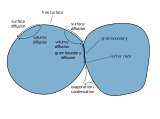
\includegraphics[height=68mm]{img/basic_theory//diffusion_mechanisms}
\end{frame}

% \begin{frame}{Overview on Sintering Modelling Approaches}
    \includegraphics[width=\textwidth]{img/numerical_methods/classification}
\end{frame}

\begin{frame}{Overview on Sintering Modelling Approaches}
    \begin{columns}
        \begin{column}{.5\textwidth}
            \begin{block}{Direct Representation}
                \begin{itemize}
                        \small
                    \item discretization of interface line
                    \item points move with evolving interface
                    \item interface tracked by point position
                \end{itemize}
            \end{block}
        \end{column}
        \begin{column}{.5\textwidth}
            \begin{block}{Indirect Representation}
                \begin{itemize}
                        \small
                    \item discretization of solution space
                    \item points fixed (except remeshing)
                    \item interface tracked by state function value
                \end{itemize}
            \end{block}
        \end{column}
    \end{columns}
    \vspace{.5em}
    \begin{columns}
        \begin{column}{.5\textwidth}
            \begin{block}{Sharp Interface}
                \begin{itemize}
                        \small
                    \item interface is sharp and unsteady jump
                    \item interface energy is localized
                    \item discretization depends on shape requirements
                \end{itemize}
            \end{block}
        \end{column}
        \begin{column}{.5\textwidth}
            \begin{block}{Diffuse Interface}
                \begin{itemize}
                        \small
                    \item interface is smooth and steady transition
                    \item interface energy is blurred
                    \item discretization depends on gradient requirements
                \end{itemize}
            \end{block}
        \end{column}
    \end{columns}
\end{frame}


\section{Sintering Model Development}

% \begin{frame}{Reasoning Behind Current Approach}
    \begin{description}
        \item[Direct Representation] allow adressing of surface relative to particle position \\
            $\rightarrow$ easy rigid body movement
        \item[Sharp Interface] have localized interface energy \\
            $\rightarrow$ have material data invariant to discretization
        \item[Finite Difference Discretization] state of particle interior not needed
        \item[Thermal Extremal Principle Solution] obtain concise near-linear equation system with implicit respect to constraints
    \end{description}
    \vspace{1em}

    \centering\structure{Discretization depends on geometry requirements, allowing rigorous remeshing to save effort in late stages.}
\end{frame}

\begin{frame}[nofoottext]{Overview: Two Particles According to the Model}
    \centering
    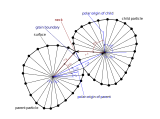
\includegraphics[height=78mm]{img/model_development/two_particle_contact}
\end{frame}

\begin{frame}[fragile]{Thermodynamic Extremal Principle}
    \begin{block}{Thermodynamic Extremal Principle}
        System evolution will follow the path of maximum dissipation with respect to all constraints.
    \end{block}

    \begin{tblr}[
            label=none,
            entry=none,
        ]{
            colspec={lX[c]},
        }
        Thermodynamic Dissipation &
        $\displaystyle \Dissipation(\Vect\ExternalStateVariable, \Vect\InternalStateVariable, \Vect{\InternalStateVelocity}) = -\frac{\partial\GibbsEnergy(\Vect\ExternalStateVariable, \Vect\InternalStateVariable, \Vect\InternalDegreeOfFreedom)}{\partial \Vect\InternalStateVariable} \cdot \Vect{\InternalStateVelocity} \rightarrow \max_{\Vect{\InternalStateVelocity}}$ \\
        Kinetic Dissipation       &
        $\displaystyle \Dissipation(\Vect\ExternalStateVariable, \Vect\InternalStateVariable, \Vect{\InternalStateVelocity}) - \DissipationFunction(\Vect\ExternalStateVariable, \Vect\InternalStateVariable, \Vect{\Flux}) = 0$  \\
        Constraints      &
        $\displaystyle \Vect\Constraint(\Vect\ExternalStateVariable, \Vect\InternalStateVariable, \Vect{\InternalStateVelocity}, \Vect\Flux, \Vect\InternalDegreeOfFreedom) = 0 $
    \end{tblr}

    \footreference{\cite{Onsager1931, Ziegler1963, Svoboda1991, Fischer2014, Hackl2020a}, \ldots}
\end{frame}

% \begin{frame}[nofoottext]{Element Geometry}
    \centering
    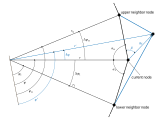
\includegraphics[height=78mm]{img/model_development/element_geometry}
\end{frame}

\begin{frame}{Normal Node Shifting}
    \centering
    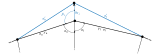
\includegraphics[width=\linewidth]{img/model_development/node_shift_normal}
    \begin{columns}
        \begin{column}{0.5\linewidth}
            \begin{equation*}
                \frac{\partial \GibbsEnergy}{\partial {\Shift}_{\Normal}} = -\left({\InterfaceEnergy}_{\Upper} + {\InterfaceEnergy}_{\Lower}\right) \cos \SurfaceVectorAngle_{\Normal}
            \end{equation*}
        \end{column}
        \begin{column}{0.5\linewidth}
            \begin{equation*}
                \frac{\partial \Volume}{\partial {\Shift}_{\Normal}} = \frac{1}{2} \left( \SurfaceDistance_{\Upper} + \SurfaceDistance_{\Lower} \right) \sin \SurfaceVectorAngle_{\Normal}
            \end{equation*}
        \end{column}
    \end{columns}
\end{frame}

\begin{frame}{Tangential Node Shifting}
    \centering
    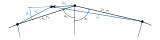
\includegraphics[width=\linewidth]{img/model_development/node_shift_tangential}
    \begin{columns}
        \begin{column}{0.5\linewidth}
            \begin{equation*}
                \frac{\partial \GibbsEnergy}{\partial {\Shift}_{\Tangential}} = \lim_{\Step\Shift_{\Tangential} \rightarrow 0} \frac{\Step\GibbsEnergy_{\Tangential}}{\Step\Shift_{\Tangential}} = -\left({\InterfaceEnergy}_{\Upper} - {\InterfaceEnergy}_{\Lower}\right) \cos \SurfaceVectorAngle_{\Tangential}
            \end{equation*}
        \end{column}
        \begin{column}{0.5\linewidth}
            \begin{equation*}
                \frac{\partial \Volume}{\partial {\Shift}_{\Tangential}} = \lim_{\Step\Shift_{\Tangential} \rightarrow 0} \frac{\Step\Volume_{\Tangential\Upper} - \Step\Volume_{\Tangential\Lower}}{\Step\Shift_{\Tangential}} = \frac{1}{2} \left( \SurfaceDistance_{\Upper} - \SurfaceDistance_{\Lower} \right) \sin \SurfaceVectorAngle_{\Tangential}
            \end{equation*}
        \end{column}
    \end{columns}
\end{frame}

\begin{frame}[nofoottext]{Contact Conditions: Absolute Node Shift}
    \centering
    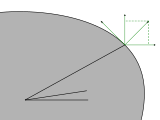
\includegraphics[height=78mm]{img/model_development/node_shift_global}
\end{frame}


\section{Two-Particle Contacts}

% \subsection{Surface-Boundary-Energy-Ratio}
% \begin{frame}{Shrinkage Evolution -- Surface-Boundary-Energy-Ratio $\InterfaceEnergy_{\GrainBoundary} / \InterfaceEnergy_{\Surface}$}
    \centering
    \includegraphics[width=\linewidth]{sim/two_particle/studies/surface_boundary_energy/shrinkage}\\
\end{frame}

% \begin{frame}{Shrinkage Evolution -- Surface-Boundary-Energy-Ratio $\InterfaceEnergy_{\GrainBoundary} / \InterfaceEnergy_{\Surface}$}
    \centering
    \includegraphics[width=\linewidth]{sim/two_particle/studies/surface_boundary_energy/shrinkage}\\
\end{frame}

% \begin{frame}{Shrinkage Evolution -- Surface-Boundary-Energy-Ratio $\InterfaceEnergy_{\GrainBoundary} / \InterfaceEnergy_{\Surface}$}
    \centering
    \includegraphics[width=\linewidth]{sim/two_particle/studies/surface_boundary_energy/shrinkage}\\
\end{frame}


% \subsection{Surface-Boundary-Diffusion-Ratio}
% \begin{frame}{Shrinkage Evolution -- Surface-Boundary-Diffusion-Ratio $\DiffusionCoefficient_{\GrainBoundary} / \DiffusionCoefficient_{\Surface}$}
    \centering
    \includegraphics[width=\linewidth]{sim/two_particle/studies/surface_boundary_diffusion/shrinkage_map}\\
\end{frame}

% \begin{frame}{Shrinkage Evolution -- Surface-Boundary-Diffusion-Ratio $\DiffusionCoefficient_{\GrainBoundary} / \DiffusionCoefficient_{\Surface}$}
    \centering
    \includegraphics[width=\linewidth]{sim/two_particle/studies/surface_boundary_diffusion/shrinkage_map}\\
\end{frame}

% \begin{frame}{Shrinkage Evolution -- Surface-Boundary-Diffusion-Ratio $\DiffusionCoefficient_{\GrainBoundary} / \DiffusionCoefficient_{\Surface}$}
    \centering
    \includegraphics[width=\linewidth]{sim/two_particle/studies/surface_boundary_diffusion/shrinkage_map}\\
\end{frame}


\subsection{Particle-Size-Ratio}
\begin{frame}{Geometry Evolution -- Particle-Size-Ratio $\Radius_2 / \Radius_1$}
    \centering
    \only<1>{%
        \includegraphics[width=\linewidth]{sim/two_particle/studies/particle_size_ratio/1.00000/evolution}\\
        $\Radius_2 / \Radius_1 = \num{1}$%
    }%
    \only<2>{%
        \includegraphics[width=\linewidth]{sim/two_particle/studies/particle_size_ratio/2.00000/evolution}\\
        $\Radius_2 / \Radius_1 = \num{2}$%
    }%
    \only<3>{%
        \includegraphics[width=\linewidth]{sim/two_particle/studies/particle_size_ratio/3.00000/evolution}\\
        $\Radius_2 / \Radius_1 = \num{3}$%
    }%
    \only<4>{%
        \includegraphics[width=\linewidth]{sim/two_particle/studies/particle_size_ratio/10.00000/evolution}\\
        $\Radius_2 / \Radius_1 = \num{10}$%
    }%
\end{frame}

\begin{frame}{Geometry Evolution -- Particle-Size-Ratio $\Radius_2 / \Radius_1$}
    \centering
    \only<1>{%
        \includegraphics[width=\linewidth]{sim/two_particle/studies/particle_size_ratio/1.00000/evolution}\\
        $\Radius_2 / \Radius_1 = \num{1}$%
    }%
    \only<2>{%
        \includegraphics[width=\linewidth]{sim/two_particle/studies/particle_size_ratio/2.00000/evolution}\\
        $\Radius_2 / \Radius_1 = \num{2}$%
    }%
    \only<3>{%
        \includegraphics[width=\linewidth]{sim/two_particle/studies/particle_size_ratio/3.00000/evolution}\\
        $\Radius_2 / \Radius_1 = \num{3}$%
    }%
    \only<4>{%
        \includegraphics[width=\linewidth]{sim/two_particle/studies/particle_size_ratio/10.00000/evolution}\\
        $\Radius_2 / \Radius_1 = \num{10}$%
    }%
\end{frame}

\begin{frame}{Geometry Evolution -- Particle-Size-Ratio $\Radius_2 / \Radius_1$}
    \centering
    \only<1>{%
        \includegraphics[width=\linewidth]{sim/two_particle/studies/particle_size_ratio/1.00000/evolution}\\
        $\Radius_2 / \Radius_1 = \num{1}$%
    }%
    \only<2>{%
        \includegraphics[width=\linewidth]{sim/two_particle/studies/particle_size_ratio/2.00000/evolution}\\
        $\Radius_2 / \Radius_1 = \num{2}$%
    }%
    \only<3>{%
        \includegraphics[width=\linewidth]{sim/two_particle/studies/particle_size_ratio/3.00000/evolution}\\
        $\Radius_2 / \Radius_1 = \num{3}$%
    }%
    \only<4>{%
        \includegraphics[width=\linewidth]{sim/two_particle/studies/particle_size_ratio/10.00000/evolution}\\
        $\Radius_2 / \Radius_1 = \num{10}$%
    }%
\end{frame}


\section{Multi-Particle Contacts}

\begin{frame}{Geometry Evolution - Triangle Packing}
    \centering
    \includegraphics[width=\linewidth]{sim/packings/cases/triangle/evolution}\\
\end{frame}

\begin{frame}{Geometry Evolution - Square Packing}
    \centering
    \includegraphics[width=\linewidth]{sim/packings/cases/square/evolution}\\
\end{frame}

\begin{frame}{Geometry Evolution - Rhombus Packing}
    \centering
    \only<1>{%
        \includegraphics[width=\linewidth]{sim/packings/cases/rhombus/evolution}\\
        \adjustbox{set depth = 0pt}{\structure{all active}}%
    }%
    \only<2>{%
        \includegraphics[width=\linewidth]{sim/packings/cases/rhombus_inert/evolution}\\
        \adjustbox{set depth = 0pt}{\structure{upper inert}}%
    }%
\end{frame}

\begin{frame}{Shrinkage}
    \includegraphics[width=\linewidth]{sim/packings/shrinkage}
\end{frame}

\begin{frame}{Average Neck Size}
    \includegraphics[width=\linewidth]{sim/packings/neck_size}
\end{frame}


\section{Statistical Powder Modeling}

\begin{frame}{Particle Description Using Shape Function}
    \begin{columns}
        \begin{column}{0.4\linewidth}
            \begin{description}
                \item[Base Function]
                    \begin{equation*}
                        \Radius\left( \Angle \right) = \Radius_0 \cdot \left[ \prod_i \ShapeFunction_i\left( \Angle \right) \right]
                        \label{eq:shape-function-general-form}
                    \end{equation*}
                \item[Ovality Shape Function]
                    \begin{equation*}
                        \ShapeFunction_{\Ovality} = \sqrt{\frac{\Ovality}{\Ovality^2 \sin^2 \Angle + \cos^2 \Angle}}
                        \label{eq:f-ovality}
                    \end{equation*}
                \item[First-Order Wave Function]
                    \begin{equation*}
                        \ShapeFunction_1 = \WaveHeight_1 \cdot \cos \left( \WaveCount_1\Angle + 2\PI \WaveShift_1\right) + 1
                        \label{eq:f-first-order-waves}
                    \end{equation*}
            \end{description}
        \end{column}
        \begin{column}{0.6\linewidth}
            \includegraphics[width=\linewidth]{img/randomized/1694_48_shape}
        \end{column}
    \end{columns}
\end{frame}

\begin{frame}{Statistical Results on Particle Morphology}
    \only<1>{
        \centering
        \includegraphics[width=\linewidth, clip, viewport=0 105mm 160mm 157.5mm]{data/morphology/batches/hist_shape/all}\\
        \vspace{1ex}
        \structure{Particle Size}\\
        Bimodal Mixed Weibull-Distribution
    }
    \only<2>{
        \begin{columns}
            \begin{column}{0.5\linewidth}
                \centering
                \includegraphics[width=\linewidth, clip, viewport=0 52.5mm 80mm 105mm]{data/morphology/batches/hist_shape/all}\\
                \vspace{1ex}
                \structure{Ovality}\\
                Weibull-Distribution
            \end{column}
            \begin{column}{0.5\linewidth}
                \centering
                \includegraphics[width=\linewidth, clip, viewport=80mm 52.5mm 160mm 105mm]{data/morphology/batches/hist_shape/all}\\
                \vspace{1ex}
                \structure{Wave Height}\\
                Beta-Distribution
            \end{column}
        \end{columns}
    }
    \only<3>{
        \begin{columns}
            \begin{column}{0.5\linewidth}
                \centering
                \includegraphics[width=\linewidth, clip, viewport=0 0 80mm 52.5mm]{data/morphology/batches/hist_shape/all}\\
                \vspace{1ex}
                \structure{Phase Shift}\\
                Uniform Distribution
            \end{column}
            \begin{column}{0.5\linewidth}
                \centering
                \includegraphics[width=\linewidth, clip, viewport=80mm 0 160mm 52.5mm]{data/morphology/batches/hist_shape/all}\\
                \vspace{1ex}
                \structure{Wave Count}\\
                Categorical Distribution
            \end{column}
        \end{columns}
    }
\end{frame}

\begin{frame}{Randomized Simulations -- Monte-Carlo Approach}
    \begin{itemize}
        \item Random sampling of radius, ovality and shape parameters for 3 distinct particles.
        \item Generation of initial contact state.
        \item Simulation till end time reached or pore closed.
        \item Repeating several hundred times and collecting results.
        \item Easy parallelization due to independent simulations.
    \end{itemize}
\end{frame}

\begin{frame}{Randomized Simulation Results -- Building a Curve Family Plot}
    \only<1>{\includegraphics[width=\linewidth, clip, viewport=0 53mm 160mm 140mm]{sim/randomized/cases/circular/shrinkage1}}
    \only<2>{\includegraphics[width=\linewidth, clip, viewport=0 53mm 160mm 140mm]{sim/randomized/cases/circular/shrinkage2}}
    \only<3>{\includegraphics[width=\linewidth, clip, viewport=0 53mm 160mm 140mm]{sim/randomized/cases/circular/shrinkage10}}
    \only<4>{\includegraphics[width=\linewidth, clip, viewport=0 53mm 160mm 140mm]{sim/randomized/cases/circular/shrinkage100}}
\end{frame}


\subsection{Shrinkage}
\begin{frame}{Randomized Simulation Results -- Neck Size -- Circular Particles}
    \includegraphics[width=\linewidth, clip, viewport=0 53mm 160mm 140mm]{sim/randomized/cases/circular/neck_size}
\end{frame}

\begin{frame}{Randomized Simulation Results -- Neck Size -- Oval Particles}
    \includegraphics[width=\linewidth, clip, viewport=0 53mm 160mm 140mm]{sim/randomized/cases/oval/neck_size}
\end{frame}

\begin{frame}{Randomized Simulation Results -- Shrinkage -- Waved Particles}
    \includegraphics[width=\linewidth, clip, viewport=0 53mm 160mm 140mm]{sim/randomized/cases/shape/shrinkage}
\end{frame}


\subsection{Neck Size}
\begin{frame}{Randomized Simulation Results -- Neck Size -- Circular Particles}
    \includegraphics[width=\linewidth, clip, viewport=0 53mm 160mm 140mm]{sim/randomized/cases/circular/neck_size}
\end{frame}

\begin{frame}{Randomized Simulation Results -- Neck Size -- Oval Particles}
    \includegraphics[width=\linewidth, clip, viewport=0 53mm 160mm 140mm]{sim/randomized/cases/oval/neck_size}
\end{frame}

\begin{frame}{Randomized Simulation Results -- Shrinkage -- Waved Particles}
    \includegraphics[width=\linewidth, clip, viewport=0 53mm 160mm 140mm]{sim/randomized/cases/shape/shrinkage}
\end{frame}


\frame[plain]{\makeclosing}

\appendix

\begin{frame}[label=appendix-contents]{Appendix Contents}
    \begin{multicols}{2}
        \tableofcontents
    \end{multicols}
\end{frame}

\section{Sintering Model Development}

\begin{frame}{Normal Node Shifting}
    \centering
    \includegraphics[width=\linewidth]{img/model_development/plot_normal_potential}
    \begin{equation*}
        \frac{\partial \GibbsEnergy}{\partial {\Shift}_{\Normal}} = -\left({\InterfaceEnergy}_{\Upper} + {\InterfaceEnergy}_{\Lower}\right) \cos \SurfaceVectorAngle_{\Normal}
    \end{equation*}
\end{frame}

\begin{frame}{Tangential Node Shifting -- Potential}
    \centering
    \includegraphics[width=\linewidth]{img/model_development/plot_tangential_potential}
    \begin{equation*}
        \frac{\partial \GibbsEnergy}{\partial {\Shift}_{\Tangential}} = \lim_{\Step\Shift_{\Tangential} \rightarrow 0} \frac{\Step\GibbsEnergy_{\Tangential}}{\Step\Shift_{\Tangential}} = -\left({\InterfaceEnergy}_{\Upper} - {\InterfaceEnergy}_{\Lower}\right) \cos \SurfaceVectorAngle_{\Tangential}
    \end{equation*}
\end{frame}


\begin{frame}{Normal Node Shifting -- Neck}
    \centering
    \includegraphics[width=\linewidth]{img/model_development/node_shift_normal_neck}
    \begin{columns}
        \begin{column}{0.5\linewidth}
            \begin{equation*}
                \frac{\partial \GibbsEnergy}{\partial {\Shift}_{\Normal}} = -\left( {\InterfaceEnergy}_{\Upper} \cos \SurfaceVectorAngle_{\Normal\Upper} - {\InterfaceEnergy}_{\Lower} \cos \SurfaceVectorAngle_{\Normal\Lower} \right)
            \end{equation*}
        \end{column}
        \begin{column}{0.5\linewidth}
            \begin{equation*}
                \frac{\partial \Volume}{\partial {\Shift}_{\Normal}} = \frac{1}{2} \left( \SurfaceDistance_{\Upper} \sin \SurfaceVectorAngle_{\Normal\Upper} + \SurfaceDistance_{\Lower} \sin \SurfaceVectorAngle_{\Normal\Lower}\right)
            \end{equation*}
        \end{column}
    \end{columns}
\end{frame}

\begin{frame}{Tangential Node Shifting -- Neck}
    \centering
    \includegraphics[width=\linewidth]{img/model_development/node_shift_tangential_neck}
    \begin{columns}
        \begin{column}{0.5\linewidth}
            \begin{equation*}
                \frac{\partial \GibbsEnergy}{\partial {\Shift}_{\Tangential}} = -\left( {\InterfaceEnergy}_{\Upper} \cos \SurfaceVectorAngle_{\Tangential\Upper} - {\InterfaceEnergy}_{\Lower} \cos \SurfaceVectorAngle_{\Tangential\Lower}\right)
            \end{equation*}
        \end{column}
        \begin{column}{0.5\linewidth}
            \begin{equation*}
                \frac{\partial \Volume}{\partial {\Shift}_{\Tangential}} = \frac{1}{2} \left( \SurfaceDistance_{\Upper} \sin \SurfaceVectorAngle_{\Tangential\Upper} - \SurfaceDistance_{\Lower} \sin \SurfaceVectorAngle_{\Tangential\Lower}\right)
            \end{equation*}
        \end{column}
    \end{columns}
\end{frame}


\section{Model Implementation}

\begin{frame}[nofoottext]{Equation System Structure}
    \centering
    \begin{columns}
        \begin{column}{0.5\linewidth}
            \begin{itemize}
                \item Non-linear equation system.
                \item Sparse symmetrical gradient matrix.
                \item Block structure regarding quantities (state variables, fluxes) and constraints (with their lambdas).
            \end{itemize}
        \end{column}
        \begin{column}{0.5\linewidth}
            \includegraphics[width=\textwidth]{img/implementation/sparse_structure}
        \end{column}
    \end{columns}
\end{frame}


\section{Two-Particle Contacts}

\subsection{Surface-Boundary-Energy-Ratio}
\begin{frame}{Shrinkage Evolution -- Surface-Boundary-Energy-Ratio $\InterfaceEnergy_{\GrainBoundary} / \InterfaceEnergy_{\Surface}$}
    \centering
    \includegraphics[width=\linewidth]{sim/two_particle/studies/surface_boundary_energy/shrinkage}\\
\end{frame}

\begin{frame}{Shrinkage Evolution -- Surface-Boundary-Energy-Ratio $\InterfaceEnergy_{\GrainBoundary} / \InterfaceEnergy_{\Surface}$}
    \centering
    \includegraphics[width=\linewidth]{sim/two_particle/studies/surface_boundary_energy/shrinkage}\\
\end{frame}

\begin{frame}{Shrinkage Evolution -- Surface-Boundary-Energy-Ratio $\InterfaceEnergy_{\GrainBoundary} / \InterfaceEnergy_{\Surface}$}
    \centering
    \includegraphics[width=\linewidth]{sim/two_particle/studies/surface_boundary_energy/shrinkage}\\
\end{frame}

\begin{frame}{Shrinkage Evolution -- Surface-Boundary-Energy-Ratio $\InterfaceEnergy_{\GrainBoundary} / \InterfaceEnergy_{\Surface}$}
    \centering
    \includegraphics[width=\linewidth]{sim/two_particle/studies/surface_boundary_energy/shrinkage}\\
\end{frame}

\begin{frame}{Shrinkage Evolution -- Surface-Boundary-Energy-Ratio $\InterfaceEnergy_{\GrainBoundary} / \InterfaceEnergy_{\Surface}$}
    \centering
    \includegraphics[width=\linewidth]{sim/two_particle/studies/surface_boundary_energy/shrinkage}\\
\end{frame}


\subsection{Surface-Boundary-Diffusion-Ratio}
\begin{frame}{Shrinkage Evolution -- Surface-Boundary-Diffusion-Ratio $\DiffusionCoefficient_{\GrainBoundary} / \DiffusionCoefficient_{\Surface}$}
    \centering
    \includegraphics[width=\linewidth]{sim/two_particle/studies/surface_boundary_diffusion/shrinkage_map}\\
\end{frame}

\begin{frame}{Shrinkage Evolution -- Surface-Boundary-Diffusion-Ratio $\DiffusionCoefficient_{\GrainBoundary} / \DiffusionCoefficient_{\Surface}$}
    \centering
    \includegraphics[width=\linewidth]{sim/two_particle/studies/surface_boundary_diffusion/shrinkage_map}\\
\end{frame}

\begin{frame}{Shrinkage Evolution -- Surface-Boundary-Diffusion-Ratio $\DiffusionCoefficient_{\GrainBoundary} / \DiffusionCoefficient_{\Surface}$}
    \centering
    \includegraphics[width=\linewidth]{sim/two_particle/studies/surface_boundary_diffusion/shrinkage_map}\\
\end{frame}

\begin{frame}{Shrinkage Evolution -- Surface-Boundary-Diffusion-Ratio $\DiffusionCoefficient_{\GrainBoundary} / \DiffusionCoefficient_{\Surface}$}
    \centering
    \includegraphics[width=\linewidth]{sim/two_particle/studies/surface_boundary_diffusion/shrinkage_map}\\
\end{frame}

\begin{frame}{Shrinkage Evolution -- Surface-Boundary-Diffusion-Ratio $\DiffusionCoefficient_{\GrainBoundary} / \DiffusionCoefficient_{\Surface}$}
    \centering
    \includegraphics[width=\linewidth]{sim/two_particle/studies/surface_boundary_diffusion/shrinkage_map}\\
\end{frame}


\subsection{Particle-Size-Ratio}
\begin{frame}{Geometry Evolution -- Particle-Size-Ratio $\Radius_2 / \Radius_1$}
    \centering
    \only<1>{%
        \includegraphics[width=\linewidth]{sim/two_particle/studies/particle_size_ratio/1.00000/evolution}\\
        $\Radius_2 / \Radius_1 = \num{1}$%
    }%
    \only<2>{%
        \includegraphics[width=\linewidth]{sim/two_particle/studies/particle_size_ratio/2.00000/evolution}\\
        $\Radius_2 / \Radius_1 = \num{2}$%
    }%
    \only<3>{%
        \includegraphics[width=\linewidth]{sim/two_particle/studies/particle_size_ratio/3.00000/evolution}\\
        $\Radius_2 / \Radius_1 = \num{3}$%
    }%
    \only<4>{%
        \includegraphics[width=\linewidth]{sim/two_particle/studies/particle_size_ratio/10.00000/evolution}\\
        $\Radius_2 / \Radius_1 = \num{10}$%
    }%
\end{frame}

\begin{frame}{Geometry Evolution -- Particle-Size-Ratio $\Radius_2 / \Radius_1$}
    \centering
    \only<1>{%
        \includegraphics[width=\linewidth]{sim/two_particle/studies/particle_size_ratio/1.00000/evolution}\\
        $\Radius_2 / \Radius_1 = \num{1}$%
    }%
    \only<2>{%
        \includegraphics[width=\linewidth]{sim/two_particle/studies/particle_size_ratio/2.00000/evolution}\\
        $\Radius_2 / \Radius_1 = \num{2}$%
    }%
    \only<3>{%
        \includegraphics[width=\linewidth]{sim/two_particle/studies/particle_size_ratio/3.00000/evolution}\\
        $\Radius_2 / \Radius_1 = \num{3}$%
    }%
    \only<4>{%
        \includegraphics[width=\linewidth]{sim/two_particle/studies/particle_size_ratio/10.00000/evolution}\\
        $\Radius_2 / \Radius_1 = \num{10}$%
    }%
\end{frame}

\begin{frame}{Geometry Evolution -- Particle-Size-Ratio $\Radius_2 / \Radius_1$}
    \centering
    \only<1>{%
        \includegraphics[width=\linewidth]{sim/two_particle/studies/particle_size_ratio/1.00000/evolution}\\
        $\Radius_2 / \Radius_1 = \num{1}$%
    }%
    \only<2>{%
        \includegraphics[width=\linewidth]{sim/two_particle/studies/particle_size_ratio/2.00000/evolution}\\
        $\Radius_2 / \Radius_1 = \num{2}$%
    }%
    \only<3>{%
        \includegraphics[width=\linewidth]{sim/two_particle/studies/particle_size_ratio/3.00000/evolution}\\
        $\Radius_2 / \Radius_1 = \num{3}$%
    }%
    \only<4>{%
        \includegraphics[width=\linewidth]{sim/two_particle/studies/particle_size_ratio/10.00000/evolution}\\
        $\Radius_2 / \Radius_1 = \num{10}$%
    }%
\end{frame}

\begin{frame}{Geometry Evolution -- Particle-Size-Ratio $\Radius_2 / \Radius_1$}
    \centering
    \only<1>{%
        \includegraphics[width=\linewidth]{sim/two_particle/studies/particle_size_ratio/1.00000/evolution}\\
        $\Radius_2 / \Radius_1 = \num{1}$%
    }%
    \only<2>{%
        \includegraphics[width=\linewidth]{sim/two_particle/studies/particle_size_ratio/2.00000/evolution}\\
        $\Radius_2 / \Radius_1 = \num{2}$%
    }%
    \only<3>{%
        \includegraphics[width=\linewidth]{sim/two_particle/studies/particle_size_ratio/3.00000/evolution}\\
        $\Radius_2 / \Radius_1 = \num{3}$%
    }%
    \only<4>{%
        \includegraphics[width=\linewidth]{sim/two_particle/studies/particle_size_ratio/10.00000/evolution}\\
        $\Radius_2 / \Radius_1 = \num{10}$%
    }%
\end{frame}

\begin{frame}{Geometry Evolution -- Particle-Size-Ratio $\Radius_2 / \Radius_1$}
    \centering
    \only<1>{%
        \includegraphics[width=\linewidth]{sim/two_particle/studies/particle_size_ratio/1.00000/evolution}\\
        $\Radius_2 / \Radius_1 = \num{1}$%
    }%
    \only<2>{%
        \includegraphics[width=\linewidth]{sim/two_particle/studies/particle_size_ratio/2.00000/evolution}\\
        $\Radius_2 / \Radius_1 = \num{2}$%
    }%
    \only<3>{%
        \includegraphics[width=\linewidth]{sim/two_particle/studies/particle_size_ratio/3.00000/evolution}\\
        $\Radius_2 / \Radius_1 = \num{3}$%
    }%
    \only<4>{%
        \includegraphics[width=\linewidth]{sim/two_particle/studies/particle_size_ratio/10.00000/evolution}\\
        $\Radius_2 / \Radius_1 = \num{10}$%
    }%
\end{frame}


\subsection{Surface-Energy-Asymmetry}
\begin{frame}{Shrinkage Evolution -- Surface-Energy-Asymmetry $\InterfaceEnergy_{\Surface2} / \InterfaceEnergy_{\Surface1}$}
    \centering
    \includegraphics[width=\linewidth]{sim/two_particle/studies/surface_energy_asymmetric/shrinkage_map}\\
\end{frame}

\begin{frame}{Shrinkage Evolution -- Surface-Energy-Asymmetry $\InterfaceEnergy_{\Surface2} / \InterfaceEnergy_{\Surface1}$}
    \centering
    \includegraphics[width=\linewidth]{sim/two_particle/studies/surface_energy_asymmetric/shrinkage_map}\\
\end{frame}

\begin{frame}{Shrinkage Evolution -- Surface-Energy-Asymmetry $\InterfaceEnergy_{\Surface2} / \InterfaceEnergy_{\Surface1}$}
    \centering
    \includegraphics[width=\linewidth]{sim/two_particle/studies/surface_energy_asymmetric/shrinkage_map}\\
\end{frame}

\begin{frame}{Shrinkage Evolution -- Surface-Energy-Asymmetry $\InterfaceEnergy_{\Surface2} / \InterfaceEnergy_{\Surface1}$}
    \centering
    \includegraphics[width=\linewidth]{sim/two_particle/studies/surface_energy_asymmetric/shrinkage_map}\\
\end{frame}

\begin{frame}{Shrinkage Evolution -- Surface-Energy-Asymmetry $\InterfaceEnergy_{\Surface2} / \InterfaceEnergy_{\Surface1}$}
    \centering
    \includegraphics[width=\linewidth]{sim/two_particle/studies/surface_energy_asymmetric/shrinkage_map}\\
\end{frame}


\subsection{Diffusion-Asymmetry}
\begin{frame}{Shrinkage Evolution -- Diffusion-Asymmetry $\DiffusionCoefficient_{2} / \DiffusionCoefficient_{1}$}
    \centering
    \includegraphics[width=\linewidth]{sim/two_particle/studies/diffusion_asymmetric/shrinkage_map}\\
\end{frame}

\begin{frame}{Shrinkage Evolution -- Diffusion-Asymmetry $\DiffusionCoefficient_{2} / \DiffusionCoefficient_{1}$}
    \centering
    \includegraphics[width=\linewidth]{sim/two_particle/studies/diffusion_asymmetric/shrinkage_map}\\
\end{frame}

\begin{frame}{Shrinkage Evolution -- Diffusion-Asymmetry $\DiffusionCoefficient_{2} / \DiffusionCoefficient_{1}$}
    \centering
    \includegraphics[width=\linewidth]{sim/two_particle/studies/diffusion_asymmetric/shrinkage_map}\\
\end{frame}

\begin{frame}{Shrinkage Evolution -- Diffusion-Asymmetry $\DiffusionCoefficient_{2} / \DiffusionCoefficient_{1}$}
    \centering
    \includegraphics[width=\linewidth]{sim/two_particle/studies/diffusion_asymmetric/shrinkage_map}\\
\end{frame}

\begin{frame}{Shrinkage Evolution -- Diffusion-Asymmetry $\DiffusionCoefficient_{2} / \DiffusionCoefficient_{1}$}
    \centering
    \includegraphics[width=\linewidth]{sim/two_particle/studies/diffusion_asymmetric/shrinkage_map}\\
\end{frame}


\subsection{Ovality -- Tip-Tip-Configuration}
\begin{frame}{Neck Size Evolution -- Ovality $\Ovality$ -- Tip-Tip-Configuration }
    \centering
    \includegraphics[width=\linewidth]{sim/two_particle/studies/ovality_tip_tip/neck_size_map}\\
\end{frame}

\begin{frame}{Neck Size Evolution -- Ovality $\Ovality$ -- Tip-Tip-Configuration }
    \centering
    \includegraphics[width=\linewidth]{sim/two_particle/studies/ovality_tip_tip/neck_size_map}\\
\end{frame}

\begin{frame}{Neck Size Evolution -- Ovality $\Ovality$ -- Tip-Tip-Configuration }
    \centering
    \includegraphics[width=\linewidth]{sim/two_particle/studies/ovality_tip_tip/neck_size_map}\\
\end{frame}

\begin{frame}{Neck Size Evolution -- Ovality $\Ovality$ -- Tip-Tip-Configuration }
    \centering
    \includegraphics[width=\linewidth]{sim/two_particle/studies/ovality_tip_tip/neck_size_map}\\
\end{frame}

\begin{frame}{Neck Size Evolution -- Ovality $\Ovality$ -- Tip-Tip-Configuration }
    \centering
    \includegraphics[width=\linewidth]{sim/two_particle/studies/ovality_tip_tip/neck_size_map}\\
\end{frame}


\subsection{Ovality -- Tip-Flank-Configuration}
\begin{frame}{Shrinkage Evolution -- Ovality $\Ovality$ -- Tip-Flank-Configuration }
    \centering
    \includegraphics[width=\linewidth]{sim/two_particle/studies/ovality_tip_flank/shrinkage_map}\\
\end{frame}

\begin{frame}{Shrinkage Evolution -- Ovality $\Ovality$ -- Tip-Flank-Configuration }
    \centering
    \includegraphics[width=\linewidth]{sim/two_particle/studies/ovality_tip_flank/shrinkage_map}\\
\end{frame}

\begin{frame}{Shrinkage Evolution -- Ovality $\Ovality$ -- Tip-Flank-Configuration }
    \centering
    \includegraphics[width=\linewidth]{sim/two_particle/studies/ovality_tip_flank/shrinkage_map}\\
\end{frame}

\begin{frame}{Shrinkage Evolution -- Ovality $\Ovality$ -- Tip-Flank-Configuration }
    \centering
    \includegraphics[width=\linewidth]{sim/two_particle/studies/ovality_tip_flank/shrinkage_map}\\
\end{frame}

\begin{frame}{Shrinkage Evolution -- Ovality $\Ovality$ -- Tip-Flank-Configuration }
    \centering
    \includegraphics[width=\linewidth]{sim/two_particle/studies/ovality_tip_flank/shrinkage_map}\\
\end{frame}


\subsection{Ovality -- Flank-Flank-Configuration}
\begin{frame}{Shrinkage Evolution -- Ovality $\Ovality$ -- Flank-Flank-Configuration }
    \centering
    \includegraphics[width=\linewidth]{sim/two_particle/studies/ovality_flank_flank/shrinkage_map}\\
\end{frame}

\begin{frame}{Shrinkage Evolution -- Ovality $\Ovality$ -- Flank-Flank-Configuration }
    \centering
    \includegraphics[width=\linewidth]{sim/two_particle/studies/ovality_flank_flank/shrinkage_map}\\
\end{frame}

\begin{frame}{Shrinkage Evolution -- Ovality $\Ovality$ -- Flank-Flank-Configuration }
    \centering
    \includegraphics[width=\linewidth]{sim/two_particle/studies/ovality_flank_flank/shrinkage_map}\\
\end{frame}

\begin{frame}{Shrinkage Evolution -- Ovality $\Ovality$ -- Flank-Flank-Configuration }
    \centering
    \includegraphics[width=\linewidth]{sim/two_particle/studies/ovality_flank_flank/shrinkage_map}\\
\end{frame}

\begin{frame}{Shrinkage Evolution -- Ovality $\Ovality$ -- Flank-Flank-Configuration }
    \centering
    \includegraphics[width=\linewidth]{sim/two_particle/studies/ovality_flank_flank/shrinkage_map}\\
\end{frame}


\section{Multi-Particle Contacts}

\begin{frame}{Geometry Evolution - Triangle Packing With Inert}
    \centering
    \includegraphics[width=\linewidth]{sim/packings/cases/triangle_inert/evolution}\\
\end{frame}

\begin{frame}{Geometry Evolution - Square Packing With Inert}
    \centering
    \includegraphics[width=\linewidth]{sim/packings/cases/square_inert/evolution}\\
\end{frame}

\begin{frame}{Geometry Evolution - Rhombus Packing With Inert}
    \centering
    \includegraphics[width=\linewidth]{sim/packings/cases/rhombus_inert/evolution}\\
\end{frame}


\section{Statistical Powder Modeling}

\subsection{Shrinkage}
\begin{frame}{Randomized Simulation Results -- Neck Size -- Circular Particles}
    % \includegraphics[width=\linewidth, clip, viewport=0 0 160mm 53mm]{sim/randomized/cases/circular/neck_size}
\end{frame}

\begin{frame}{Randomized Simulation Results -- Neck Size -- Oval Particles}
    \includegraphics[width=\linewidth, clip, viewport=0 0 160mm 53mm]{sim/randomized/cases/oval/neck_size}
\end{frame}

\begin{frame}{Randomized Simulation Results -- Neck Size -- Waved Particles}
    \includegraphics[width=\linewidth, clip, viewport=0 0 160mm 53mm]{sim/randomized/cases/shape/neck_size}
\end{frame}


\subsection{Neck Size}
\begin{frame}{Randomized Simulation Results -- Neck Size -- Circular Particles}
    % \includegraphics[width=\linewidth, clip, viewport=0 0 160mm 53mm]{sim/randomized/cases/circular/neck_size}
\end{frame}

\begin{frame}{Randomized Simulation Results -- Neck Size -- Oval Particles}
    \includegraphics[width=\linewidth, clip, viewport=0 0 160mm 53mm]{sim/randomized/cases/oval/neck_size}
\end{frame}

\begin{frame}{Randomized Simulation Results -- Neck Size -- Waved Particles}
    \includegraphics[width=\linewidth, clip, viewport=0 0 160mm 53mm]{sim/randomized/cases/shape/neck_size}
\end{frame}


\end{document}
